\documentclass{article} 
\usepackage{amsmath}
\usepackage{amssymb}
\usepackage{graphicx}
\usepackage{hyperref}
\topmargin -1 cm
\headheight 0cm
\headsep 0cm
\textheight 25 cm
\textwidth 16 cm
\oddsidemargin 0 cm
\evensidemargin 0 cm
\parindent 0 pt
\parskip\smallskipamount
\usepackage{fontspec}
\setmainfont[Ligatures=TeX]{Droid Sans}
\hypersetup{
    colorlinks=true,
    linkcolor=blue,
    filecolor=magenta,      
    urlcolor=cyan,
    pdftitle={Probability and Statistics B, Project},
    bookmarks=true,
}
\begin{document}
\pagenumbering{gobble}
\begin{center}
\textbf{\huge Probability and Statistics B}\\
\textbf{\LARGE Project}\\
\textbf{\large Cameron, Duncan J}\\
\end{center}
\tableofcontents
\newpage
\pagenumbering{arabic}
\section{Hypothesis}
The task given was to investigate the difference in runtimes of Hollywood and Bollywood films, based on a criticism by a reviewer that Bollywood films are sometimes too long.\\
Hypotheses are set out as:\\
H$_\text{0}:\mu_\text{H}=\mu_\text{B}$\\
H$_\text{1}:\mu_\text{H}<\mu_\text{B}$\\
As such, an investigation is set up to see if it is fair to say that films from both categories, in general, are of the same length. If this is rejected, it is then asserted that Bollywood films are indeed longer than Hollywood films.
\section{Data}
To ensure the investigation was fair, care was taken to ensure the samples were fair and accurate reflections of the categories.
\subsection{Choice}
For the samples, 50 films from each category were selected based on the same criteria, that being:
\begin{itemize}
\item they had a release date in 2015, 2016, 2017, 2018, or 2019
\item they were in the top 10 highest grossing films of that category for their release year
\end{itemize}
The reasoning behind this decison was that revenue generated from a film is a direct measure of interest by the general public. We posture that reasons for interest in films is the same worldwide, and that the attitudes towards runtime do not change between Hollywood and Bollywood films.
\subsection{Source}
To ensure the accuracy of data, the top 10 grossing films were obtained from Wikipedia, and cross checked these with other sources. These were added to online lists in the TMDb (The Movie Database) website. TMDb is used by over 200,000 web developers to obtain information about digital media, including films, television programmes and shorts. This information includes the runtime of films, and it was these runtimes that were used in the project.\\
\textit{All sources can be found in \hyperref[sec:ref]{References}.}
\subsection{Storage}
To avoid the monotonous task of manually entering the details of 100 films, the names of the films were inserted into the online list on TMDb. TMDb has an API (Application Programming Interface) that allows information to be fetched in JSON (JavaScript Object Notation) format, which can be used in R with the \texttt{jsonlite} library. An \hyperref[sec:films]{R script} was, therefore, written to use the API to fetch the lists from the internet. These lists were stored in variables named \texttt{hollywood} and \texttt{bollywood}. Then, writing another \hyperref[sec:runtime]{R script} obtained the runtimes of each film, and stored these in vectors \texttt{hollywood\_runtime} and \texttt{bollywood\_runtime}. These were then convered to \texttt{numeric} format (from \texttt{integer} format) to allow use with R functions.
\section{Analysis}
The analysis tests the hypothesis to the 95\% and 99\% confidence intervals. This suggests that the probability of a type I error, that is the chance a correct null hypothesis is rejected, is $0.05$ and $0.01$, respectively. We first discuss if H$_\text{0}$ is true, and then consider the alternative H$_\text{1}$.
\subsection{Assumptions}
The Central Limit Theorem can be used to assume the two samples of independent film runtimes are normally distributed. This allows the use of, as the sample is large, the normal assumption to derive confidence intervals. Discussion of the validity of this assumption for the samples leads to acceptance, as below.\\
It can be seen from the histogram and Q-Q plot of normal quantiles for \hyperref[sec:hollywood]{Hollywood} films that the sample approachs a normal distribution. There is a distinctive bell shape in the histogram, and the Q-Q plot approaches a linear curve (an indicator of a normally distributed sample). There is one outlier, which may increase the mean - noted for later.\\
The plots for \hyperref[sec:bollywood]{Bollywood} films also show that we approach a normal distrinution. The samples approach a bell curve, and the Q-Q plot is relatively linear. We note that the sample does tend to favour lower film runtimes - which is again noted for later.
\subsection{Testing for H$_\text{0}$}
The 95\% and 99\% confidence intervals were obtained to test if the means are equal. Using the assumption of normally distributed samples, the test statistic can be used, that is:
$$\frac{(\bar{X}_H-\bar{X}_B)-(\mu_H-\mu_B)}{\sqrt{\frac{\sigma_H^2}{n}+\frac{\sigma_B^2}{n}}} \sim N(0,1)$$
With large $n$, take $\sigma^2=s^2$. As $s_H^2=366.1229$ and $s_B^2=214.8608$, this gives:
$$\frac{(125.5-150.42)}{\sqrt{\frac{366.1229}{50}+\frac{214.8608}{50}}}=-7.257169$$
From the $N(0,1)$ distribution, there is a 95\% confidence interval of $(-1.959964,1.959964)$. It is clear the test statistic is outwith this interval, so H$_\text{0}$ is rejected at 5\% chance of type I error.\\
A 99\% confidence interval from a $N(0,1)$ distribution is $(-2.575829,2.575829)$. Again, it is clear the test statistic is outwith this interval, so, again, reject H$_\text{0}$, this iteration with 1\% chance of type I error.
\subsection{Accepting H$_\text{1}$}
To test whether H$_\text{1}$ is acceptable as an alternative hypothesis, t-tests were ran in R at \hyperref[sec:95]{95\%} and \hyperref[sec:99]{99\%} confidence levels, on the basis of a one-sided test, that $\mu_H<\mu_B$.\\
Both tests gave a p-value of $6.327\times10^{-11}$, which suggests a very strong inclination to reject H$_\text{0}$, as it is well below the significance level, and to favour H$_\text{1}$ as an alternative hypothesis.
\section{Conclusion}
In conclusion, a fair and sufficiently large sample of Bollywood and Hollywood movies was selected. These were then applied to the hypothesis set by the film reviewer, and both confidence intervals and t-tests were used to discuss the validity of the hypothesis. The results gave, at over 99\% confidence, that Bollywood films from the sample are longer than Hollywood films. This is including a skewness due to outliers that may see the samples converge to the same mean, stregthening the statistical test.\\
Given the choice of sample and these results, it can be said that, statistically, Bollywood films are longer than Hollywood films.
\newpage
\section{References}
Throughout the project, the course notes were referred to. Alongside this, the following websites were used for consultation and to obtain data:\\
\begin{center}\begin{tabular}{ @{}c@{}c@{} }
Wikipedia&\quad(\url{https://en.wikipedia.org})\\
TMDb&\quad(\url{https://www.themoviedb.org})\\
Box Office Mojo&\quad(\url{https://www.boxofficemojo.com/})\\
Bollywood Hungama&\quad(\url{https://www.bollywoodhungama.com})\\
Khan Academy&\quad(\url{https://www.khanacademy.org})\\
Stack Overflow&\quad(\url{https://stackoverflow.com})\\
Stack Exchange&\quad(\url{https://stackexchange.com})
\end{tabular}\end{center}
\label{sec:ref}
\newpage
\appendix
\section{Films}
The data used in the two samples is given as follows.
\subsection{Hollywood}
\label{sec:hollywood}
All the movies and corresponding data can be viewed at \url{https://www.themoviedb.org/list/138881}.\\
The runtimes of movies (in order), stored in the \texttt{hollywood\_runtime} vector, are:
\begin{center}\begin{tabular}{ |c|c|c|c|c|c|c|c|c|c| }
\hline
181&118&142&104&100&124&129&128&122&123\\
\hline
134&149&118&129&144&121&90&148&119&135\\
\hline
152&129&141&119&137&133&135&131&96&120\\
\hline
133&97&147&87&106&108&109&151&123&108\\
\hline
136&124&141&95&137&91&137&141&123&148\\
\hline
\end{tabular}\end{center}
These data can be shown on a histogram:
\begin{center}
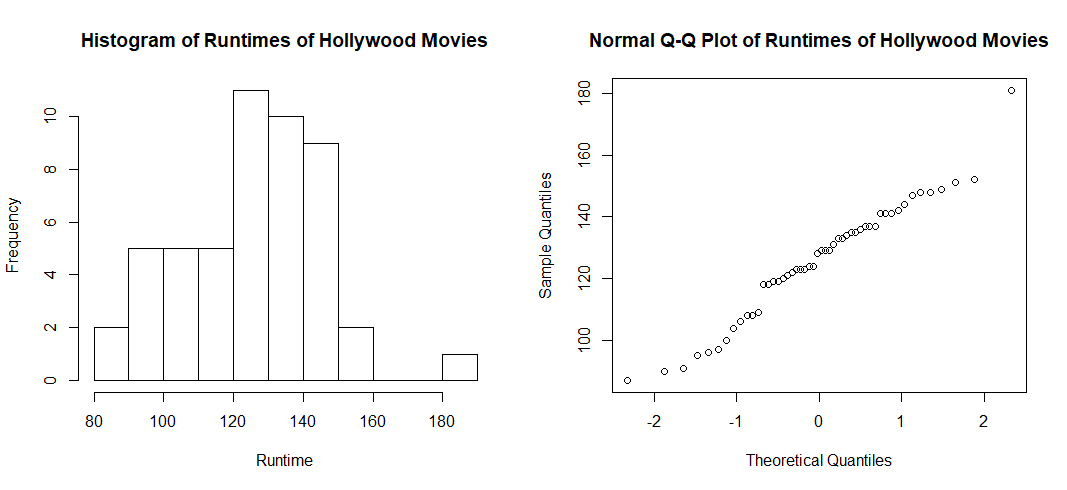
\includegraphics[scale=0.6]{hollywood_runtime.png}
\end{center}
\subsection{Bollywood}
\label{sec:bollywood}
All the movies and corresponding data can be viewed at \url{https://www.themoviedb.org/list/138884}.\\
The runtimes of movies (in order), stored in the \texttt{bollywood\_runtime} vector, are:
\begin{center}\begin{tabular}{ |c|c|c|c|c|c|c|c|c|c| }
\hline
156&171&175&138&155&132&133&142&150&161\\
\hline
164&139&159&164&160&145&140&125&140&150\\
\hline
165&132&155&151&143&150&139&136&139&161\\
\hline
158&150&190&126&140&138&153&133&159&174\\
\hline
158&158&128&153&154&170&160&123&156&170\\
\hline
\end{tabular}\end{center}
The movie \textbf{Sultan} was included in the sample, but was not in the database used. The runtime for this movie was sourced separately from Wikipedia (and cross checked) and is the final entry in the table.
\newpage
These data can be shown on a histogram:
\begin{center}
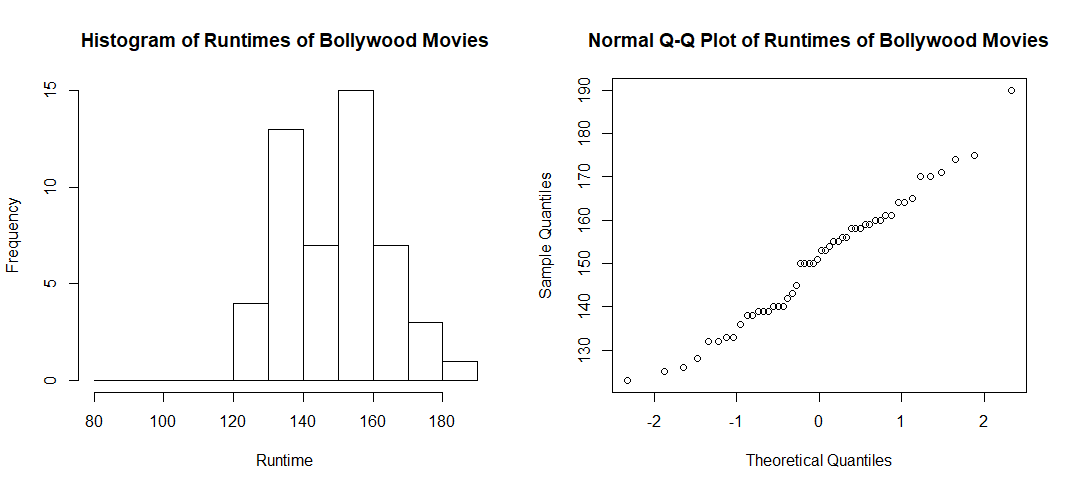
\includegraphics[scale=0.6]{bollywood_runtime.png}
\end{center}
\section{R Scripts}
These scripts are written as if querying for the Hollywood movies, they can and were simply adapted for Bollywood movies by changing references to \texttt{hollywood} to \texttt{bollywood}.
\subsection{Films}
\label{sec:films}
\texttt{hollywood\_file="https://api.themoviedb.org/3/list/138881?api\_key=\\8e2981306aaa0d1218f9fbf7165f99d8\&language=en-US"}\\\\
\texttt{\#ensure the jsonlite library is loaded\\
hollywood <- fromJSON(hollywood\_file,flatten=TRUE)\\
hollywood\_list <- hollywood['items']}
\subsection{Runtime}
\label{sec:runtime}
\texttt{\#ensure the jsonlite library is loaded\\
for(i in 1:50)\{\\
\quad id=hollywood\_list[["items"]][["id"]][[i]]\\
\quad json <- fromJSON(paste("https://api.themoviedb.org/3/movie/",id,"?api\_key=\\8e2981306aaa0d1218f9fbf7165f99d8\&language=en-US"),flatten=TRUE)\\
\quad hollywood\_runtime[i]=json['runtime']\\
\}}
\section{t-tests}
t-tests were run in R, and the outputs are given below.
\subsection{95\%}
\label{sec:95}
Running the command \texttt{t.test(hollywood\_runtime,bollywood\_runtime,alternative="l")} yielded:\\\\
\texttt{Welch Two Sample t-test\\
\\
data:  hollywood\_runtime and bollywood\_runtime\\
t = -7.205, df = 91.779, p-value = 7.9e-11\\
alternative hypothesis: true difference in means is less than 0\\
95 percent confidence interval:\\
      -Inf -18.89591\\
sample estimates:\\
mean of x mean of y\\ 
   125.86    150.42}
\subsection{99\%}
\label{sec:99}
Running the command \texttt{t.test(hollywood\_runtime,bollywood\_runtime,alternative="l"),conf.level=0.99)} yielded:\\\\
\texttt{Welch Two Sample t-test\\
\\
data:  hollywood\_runtime and bollywood\_runtime\\
t = -7.205, df = 91.779, p-value = 7.9e-11\\
alternative hypothesis: true difference in means is less than 0\\
99 percent confidence interval:\\
      -Inf -16.48918\\
sample estimates:\\
mean of x mean of y\\
   125.86    150.42}
\end{document}